\setAuthor{}
\setRound{lõppvoor}
\setYear{2019}
\setNumber{G 7}
\setDifficulty{7}
\setTopic{TODO}

\prob{3 ruutu}
\begin{wrapfigure}[4]{r}{0.45\textwidth}
  \vspace{-15pt}
  \begin{center}
  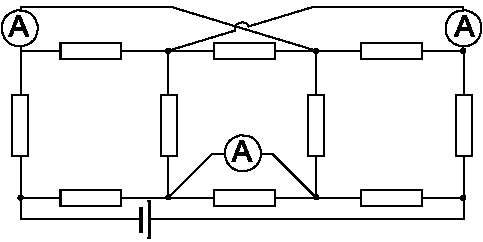
\includegraphics[scale=0.65]{2019-v3g-07-yl.pdf}
  \end{center}
  \vspace{-20pt}
\end{wrapfigure}



Toodud skeemis on kõigi takistite takistus kolm oomi, patarei pinge on 48 volti. Leidke ampermeetrite näidud. 
\vspace{25pt}



\hint

\solu
Lihtsustame skeemi arvestades sellega, et ideaalsete ampermeetrite sisetakistus on null: me võime lühistada need sõlmpunktid, mis on ühendatud juhtmega läbi ampermeetri. Selleks, et olla kindel vigadeta skeemi teisendamises tähistame takistid numbritega ja sõlmpunktid tähtedega, vt esimene joonis. Paneme tähele, et Kirchoffi vooluseaduse tõttu näitavad ampermeetrid vastavalt esimese ja viienda, seitsmenda ja neljanda ning kaheksanda ja neljanda  takisti voolude vahet.

Seejärel alustame sõlmpunktide märkimisest ja ühendame need samade takistitega, mis algseski skeemis, tulemus on näidatud teisel joonisel. Viimase sammuna  jagame sõlmpunkti C kaheks osaks lõigates mõtteliselt läbi joonise sümmeetriateljel oleva vertikaalse juhtme; seda võib teha,  sest sümmeetria tõttu puudub selles vertikaalses juhtmes vool. Nüüd on juba lihtne leida takistite voolud: takistitest 8 ja 9 koosneva ahela kogutakistus on $r_8=\SI {6}\ohm$, seetõttu  läbib neid vool $i_8=\mathcal E/r_8=\SI 8A$. Punktide B ja D vahelise viiest takistist koosneva ahelajupi takistus on $\frac 67\SI {}\ohm$ ning seega ülemise ahelapoole kogutakistus on $r_1=\frac {48}7\SI {}\ohm$ ja takisti 1 vool $i_1=\mathcal E/r_1=\SI 7A$. Seega langeb takistite 1 ja 7 peale kokku pinge $2i_1R=\SI {42}V$, mistõttu sõlmede B ja D vaheline pinge on $V_5=\mathcal E-2i_1R=\SI {6}V$. Järelikult on takisti 5 vool $i_5=V_5/R=\SI 2\A$ ja takisti 2 vool $i_2=V_5/(2R)=\SI 1\A$. 

Niisiis on vasakpoolse ülemise ampermeetri vool $i_8=i_1-i_5=\SI 5A$ ning sümmeetria tõttu näitab sama voolutugevust ka parempooolne ülemine
 
ampermeeter. Alumise ampermeetri näit on $i_8-i_2=\SI 7A$.\\

\begin{figure}[h]
    \centering
    \begin{subfigure}[h]{0.45\textwidth}
     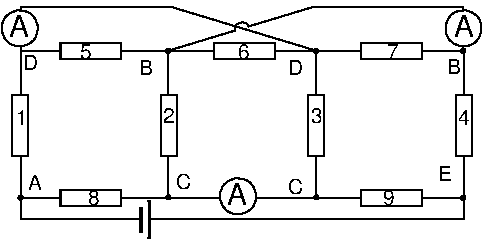
\includegraphics[width=\textwidth]{2019-v3g-07-sol1.pdf}\\
    \end{subfigure}
    \begin{subfigure}[h]{0.45\textwidth}
    \vspace{-10pt}
     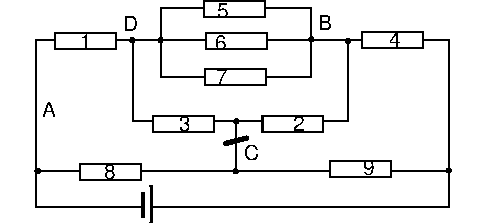
\includegraphics[width=\textwidth]{2019-v3g-07-sol2.pdf}
    \end{subfigure}
 \end{figure}
\probend